\section{Grafos eulerianos}

\subsection{As sete pontes de Königsberg}

\begin{wrapfigure}{r}{0.5\textwidth} 
    \centering
    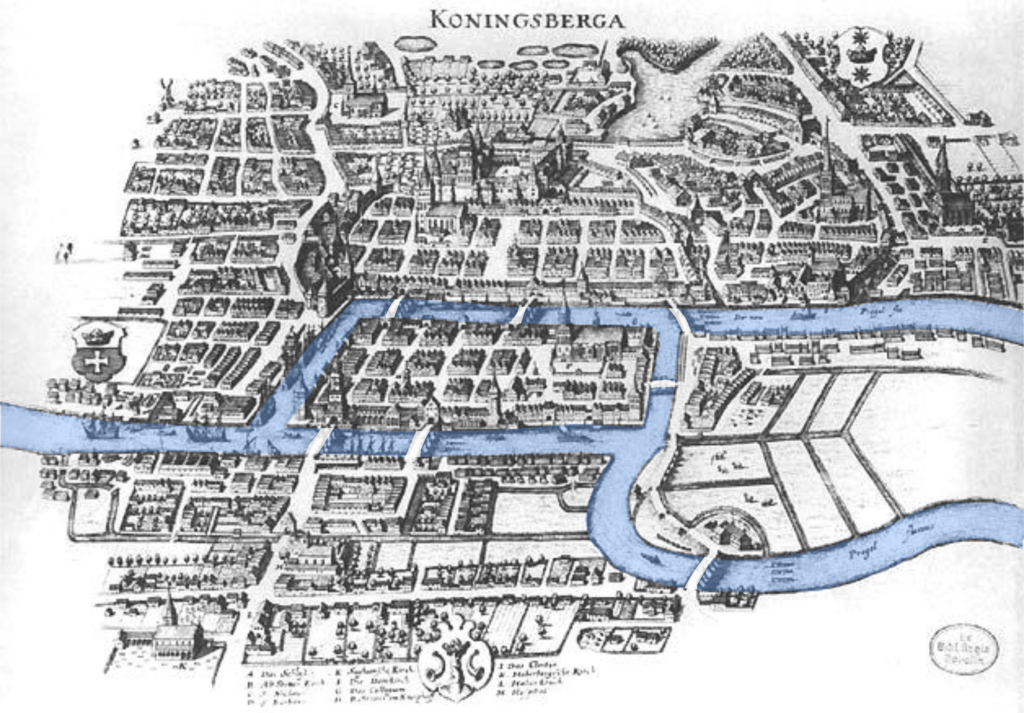
\includegraphics[width=0.5\textwidth]{konigsberg.png}
    \caption{Representação das sete pontes de Königsberg}
\end{wrapfigure}

O pro\-blema das sete pontes de Kö\-nigsberg foi des\-crito e solucio\-nado pelo matemático Leonhard Eu\-ler em 1736. 
O problema consistia em decidir se seria possível traçar no mapa de Königsberg um trajeto que percorresse cada uma de suas 7 pon\-tes uma única vez, sem repetições.

Euler resolveu esse problema do seguinte modo: 
Primeiramente, ele identificou cada uma das massas de terra do mapa com as letras A, B, C e D.

Em seguida, ele definiu que um trajeto nesse mapa seria descrito por uma sequência dessas letras: por exemplo, ``ACD'' indicaria o trajeto que se inicia na massa de terra A, move-se para a massa de terra C, usando uma das pontes, e termina na massa D.

\begin{wrapfigure}{l}{0.4\textwidth} 
    \centering
    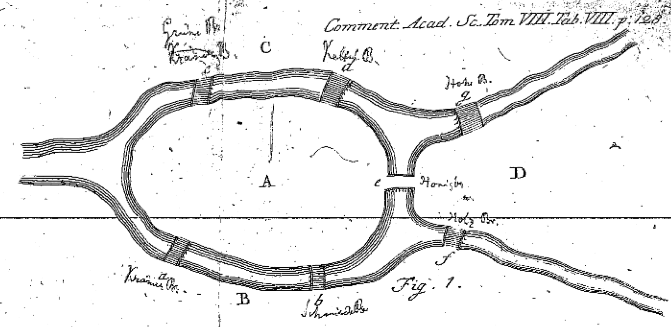
\includegraphics[width=0.4\textwidth]{konigsberg-euler.png}
    \caption{Representação de Euler}
	\label{konigsberg-euler}
\end{wrapfigure}

Euler então começou a definir algumas restrições, assumindo que o problema possuiria alguma solução:

Como o trajeto final deverá passar por todas as 7 pontes exatamente uma vez, isso implica que a sequência de letras que o representa deverá ter tamanho 8.

Além disso, como a massa de terra A possui 5 pontes, necessariamente a letra A aparecerá exatamente 3 vezes na sequência.
A massa B, C e D, no entanto possuem 3 pontes, portanto, suas letras correspondentes deverão aparecer apenas 2 vezes na sequência. 

Chegamos assim a um absurdo, pois provamos que a sequência de letras que representa uma solução deveria ter tamanho 8 e 9.
Provando assim que não existe um trajeto como o pedido no enunciado do problema.

Essa observação que, aos olhos de hoje, parece muito simples, teve um impacto profundo nas áreas da Matemática e Computação.
A modelagem de Euler, tratando as massas de terra e pontes de forma abstrata foi absolutamente inovadora e é o embrião da área da teoria dos grafos.

\subsection{Grafos não direcionados}

Antes de voltar ao problema de Euler, realizaremos algumas definições de teoria dos grafos.

Define-se como \textbf{passeio} em um grafo uma sequência finita não vazia $P = \{ v_0, v_1, \dots, v_k\}$, cujos termos são vértices $v_i$ tais que, para todo $i$, $0 \leq i < k$, os vértices $v_{i}$ e $v_{i+1}$ são ligados por uma aresta. 
Os vértices $v_0$ e $v_k$ são a origem e o término de $P$, respectivamente; e os vértices $v_1, v_2, \dots, v_{k-1}$ são chamados vértices internos de P. 

Uma \textbf{trilha} é um passeio sem arestas repetidas enquanto que um \textbf{caminho} é um passeio sem vértices repetidos.
Definimos o comprimento de um passeio, denotado por $||P||$, como o número de arestas de $P$.

Um passeio é considerado \textbf{fechado} se sua origem e término são iguais.

Uma trilha fechada é um \textbf{circuito}.

Devido às contribuições de Euler ao problema descrito, chama-se \textbf{trilha euleriana} como uma trilha que passa por todas arestas de um grafo e \textbf{grafo euleriano} como um grafo que possui um circuito euleriano fechado.

\begin{wrapfigure}{l}{0.4\textwidth}
    \centering
    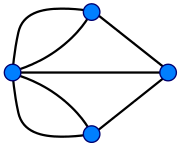
\includegraphics[width=0.3\textwidth]{konigsberg-graph.png}
    \caption{Grafo de Königsberg}
    \label{konigsberg-graph}
\end{wrapfigure}

Euler modelou essa área da cidade como um grafo, representado na figura \ref{konigsberg-graph}, tratando as pontes como arestas e as massas de terra como vértices.

A partir de tal modelagem e das definições feitas, o problema das pontes de Königsberg consiste, em definir se o grafo que representa a cidade possui ou não uma trilha euleriana. 

Apesar de ter recebido grande parte do crédito histórico pelas suas implicações, Euler não provou que qualquer grafo conexo com vértices de grau par é euleriano, essa prova só foi publicada mais de cem anos depois, em 1873, por Carl Hierholzer \cite{hierholzer}, no que se tornou o conhecido Teorema de Euler.


\begin{theorem}[Teorema de Euler ou de Euler-Hierholzer]
    Um grafo é euleriano se, e somente se, é conexo e todos seus vértices possuem grau par.
    \label{euler}
\end{theorem}

Para suportar a prova de tal teorema, primeiramente apresentaremos o seguinte lema:

Seja $\delta(G)$ o \textbf{grau mínimo} de um vértice pertencente a $G$.

\begin{lemma}
	Se $G$ é um grafo tal que $\delta(G) \geq 2$, então $G$ possui um circuito.
	\label{lema}
\end{lemma}

\begin{proof}
	Vamos assumir que um grafo qualquer $G = \{V, A\}$ não possui um caminho fechado. 
	Seja $P$ um caminho de comprimento maximal pertencente a $G$, denominamos $v$ um dos extremos de $P$. 
	Como $P$ é um caminho de comprimento maximal, é impossível, por definição, que $v$ possua uma aresta $vu$ que o ligue a um vértice $u$ não pertencente a $P$.
	
	Como, da premissa, todos vértices possuem grau maior ou igual a 2, isso implica que $v$ possuirá ao menos duas arestas que o ligam a vértices pertencentes a $P$.

	Porém, como $v$ é um vértice extremo de $P$, apenas uma dessas arestas pode pertencer ao caminho $P$. Isso implica que a outra aresta, digamos $vw$, não pertencente a $P$, implica na existência de um caminho fechado.

	Basta tomar o subcaminho entre os vértices $v$ e $w$ pertencente à $P$ juntamente com a aresta $vw$ que teremos um caminho fechado. Chegando assim em uma contradição.

	Demonstra-se assim que $G$ deverá possuir ao menos um caminho fechado dadas as condições do lema.
\end{proof}

Provado tal lema, podemos agora provar o teorema \ref{euler}:

\begin{proof}

Seja $G = \{V, E\}$ o grafo em questão.

($\Rightarrow$) Começamos provando que se um grafo é euleriano então todos seus vértices possuem grau par.

Seja $T$ um circuito euleriano, cuja existência é garantida já que $G$ é euleriano. Analisaremos o grau de um vértice qualquer $v$ de $G$.

Se $v$ não for um vértice extremo de $T$, então sempre que o mesmo aparecer em $T$ ele deverá ser precedido e sucedido de arestas, indicando assim que $v$ deverá possuir um grau par.

Do contrário, se $v$ for o vértice extremo de $T$ ele necessariamente possui duas arestas, uma ligando-o ao segundo vértice do circuito, e outra o ligando ao penúltimo vértice de $T$. 
Além disso, cada aparição de $v$ como vértice interno de $T$ contabiliza mais duas arestas ao vértice em questão, de modo que $v$ possuirá um grau par ao final.

Sendo assim, se $G$ é euleriano, então todos seus vértices (extremos ou não) possuem grau par, como queriamos demonstrar.

($\Leftarrow$) Agora, provaremos por indução no número de arestas de $G$ que se o grafo for conexo e se todos seus nós possuem grau par, então ele é euleriano.

O caso base da indução é quando não há arestas em $G$. 
O único grafo conexo que respeita tal condição é o grafo que possui apenas um vértice $v$.
Neste exemplo, $\{v\}$ é o circuito euleriano do grafo.

A hipótese de indução é que todo grafo simples, conexo, que possui até $k-1$ arestas e cujos vértices têm grau par é euleriano. 
Seja $G$ um grafo conexo, de vértices de grau par e que possua $k > 1$ arestas, provaremos que ele também deverá ser euleriano.

Como $G$ é conexo, vale que $\delta(G) \geq 1$ e como todos nós de $G$ têm grau par, podemos afirmar que $\delta(G) \geq 2$. 
Sendo assim, pelo lema \ref{lema}, $G$ deverá possuir um circuito $C$.

Se $C$ possui todas arestas de $G$, então $C$ é um circuito euleriano do grafo, finalizando a prova.

Do contrário, aplicamos o seguinte procedimento para constuir um circuito euleriano $\mathcal{C}$ de $G$:

Retira-se de $G$ as arestas pertencentes a $C$, resultando assim em um grafo $G'$. 
Possivelmente $G'$ será desconexo, por isso definimos que $G'$ será a união de $k$ componenetes conexas $G'_1, G'_2, \dots, G'_k$ disjuntas entre si.

O grau dos vértices dessas componenentes $G'_i$ deverá ser par, já que, ao retirar todas as arestas de um circuito do grafo $G$, diminuímos o grau de um vértice qualquer $v$ em duas vezes o número de aparições do mesmo no circuito. mantendo assim a paridade dos graus. 

Além disso, cada componenete conexa de $G'$ possuirá uma quantidade de arestas menor do que $k$.
Portanto, pela hipótese da indução, cada uma dessas componentes deverá possuir um circuito euleriano próprio. 
Chamaremos de $C_i$ o circuito euleriano da componente $G'_i$.

\sloppy Ao longo do algoritmo, os circuitos $C_i$ serão adicionados, um a um, ao circuito resultante $\mathcal{C}$. 
Definimos $\mathcal{T}$, como o conjunto dos circuitos eulerianos $C_i$ que ainda não fazem parte de $\mathcal{C}$. 
Inicialmente, $\mathcal{T}$ é igual ao conjunto $\{C_1, C_2, \dots, C_k\}$.


\[
	C = \{v, v_2, \dots, v_n, v\}
\]

Para cada vértice $u$ de $C$ devemos realizar as seguintes verificações:

\begin{tcolorbox}

Começamos adicionando $u$ ao circuito euleriano $\mathcal{C}$ que estamos construindo.

Enquanto houver um circuito euleriano $C_i$ pertencente a $\mathcal{T}$ do qual $u$ faz parte, fazemos o seguinte:


\begin{enumerate}
    \item Representamos $C_i$ como: 
    \[
        C_i = \{u, u_2, \dots, u_l, u\}
    \]

\item Adicionamos ao final de $\mathcal{C}$ o circuito $C_i$ como representado, exceto pelo primeiro vértice $u$. 

\item Removemos de $\mathcal{T}$ o circuito $C_i$, indicando que o mesmo já foi adicionado a $\mathcal{C}$.

\end{enumerate}

Repetem-se então as mesmas verificações para os próximos vértices de $C$.
\end{tcolorbox}


Ao final desse procedimento, o conjunto $\mathcal{T}$ deverá ser vazio, já que toda trilha $C_i$ possui pelo menos um vértice em $C$. Além disso, toda trilha $C_i$ deverá ter sido adicionada à $\mathcal{C}$ uma única vez, já que logo após adicionar uma trilha à $\mathcal{C}$ já a removiamos de $\mathcal{T}$, impedindo que ela fosse adicionada outra vez na trilha euleriana final.

Comprovado o passo da indução, finalizamos a prova do Teorema de Euler por indução.

\end{proof}

\begin{corollary}
    Um grafo possui uma trilha euleriana se, e somente se, é conexo e possui apenas zero ou dois vértices de grau ímpar.
\end{corollary}

\begin{proof}
    Seja $G$ um grafo conexo qualquer. Realizaremos a demonstração para os seguintes casos:
    \begin{enumerate}
        \item $G$ não possui vértices de grau ímpar. Neste caso, $G$ possui, segundo o teorema \ref{euler}, um circuito euleriano, e portanto, uma trilha euleriana.
        
        \item $G$ possui apenas um vértice de grau ímpar. 
			Este caso é impossível de se acontecer, já que a soma do grau de todos vértices deve ser par, impossibilitando assim que apenas um vértice tenha grau ímpar.
        
        \item $G$ possui dois vértices de grau ímpar. 

			Sejam $u$ e $v$ os únicos vértices de $G$ que possuem grau ímpar.
			Adiciona-se uma aresta fictícia ao grafo $G$, a aresta $uv$, fazendo com que tanto $u$ quanto $v$ possuam graus pares. 
			Chamaremos o grafo $G$ acrescido da aresta $uv$ de $G'$.
			Como $u$ e $v$ eram os únicos vértices de grau ímpar de $G$, vale que todos vértices de $G'$ possuirão grau par. 
			Além disso, vale que $G'$ é conexo, pois faz parte da premissa que o grafo original $G$ era conexo.

			Sendo assim, podemos aplicar o teorema \ref{euler}, provando a existência de um circuito euleriano $G'$, que chamaremos de $C$.
            Por ser euleriano, $C$ deverá percorrer a aresta $uv$ inserida, portanto podemos representar $C$ com $u$ e $v$ lado a lado, do seguinte modo:
		
			\[
				C = \{u, v, w_1, w_2, \dots, w_k, u\}
			\]


            Tome, agora, $T$ igual ao circuito $C$ sem seu vértice inicial:

            \[
                T = \{v, w_1, w_2, \dots, w_k, u\}
			\]

            Tal procedimento retira do circuito $C$ a aresta artificial $uv$, transfor\-mando-o em uma trilha $T$, que percorre todas arestas de $G`$ exceto $uv$, sendo portanto uma trilha euleriana do grafo $G$.

        \item $G$ possui três ou mais vértices de grau ímpar. 

			Assuma que existe uma trilha euleriana $T$ para $G$. 
			Neste caso, como pelo menos 3 vértices possuem grau ímpar, necessariamente existirá um vértice $v$ que não é nem o primeiro nem o último vértice de $T$.
			Isso implica que todas aparições de $v$ em $T$ são internas ao caminho, ou seja, toda aparição de $v$ será precedida e sucedida de arestas ligadas a $v$.
			Como estamos tratando de uma trilha euleriana, sabemos que todas arestas adjacentes a $v$ estão presentes em $T$ uma única vez. 
			Mas como todas arestas de $v$ devem aparecer em pares (precedendo e sucedendo $v$), isso implica que o grau de $v$ deverá ser par.
			Contradizendo a premissa.

			Por essa contradição provamos que $G$ não possuirá trilha euleriana se tiver três ou mais vértices de grau ímpar.
    \end{enumerate}
\end{proof}

% Grafos direcionados
\subsection{Grafos direcionados}

Até então tratamos apenas de grafos não direcionados, mas podemos expandir esses mesmos conceitos para grafos direcionados, os \textbf{digrafos}.

Um grafo é direcionado quando suas arestas são orientadas, chamaremos de \textbf{arcos} tais arestas. 

Numa analogia com trânsito, uma aresta é como uma estrada de mão dupla, pode-se percorrê-la nos dois sentidos, enquanto isso, um arco é como uma rua de mão única, em que apenas um sentido é permitido.

Quanto tratamos de grafos direcionados (ou digrafos), é necessário refinar a noção de grau de um vértice:
Por isso, denominamos \textbf{grau de saída} de um vértice $v$, $\delta^-(v)$, como o número de arcos que saem de $v$, e \textbf{grau de entrada}, $\delta^+(v)$, como o número de arcos que entram em $v$. 

Definimos como \textbf{fortemente conexo} um digrafo que possui um caminho entre todo par de vértices, e como \textbf{fracamente conexo} um digrafo que possui para todo par de vértices $u$ e $v$ um caminho de $u$ a $v$ ou de $v$ a $u$.

Dadas as devidas definições, apresentamos agora o teorema de Euler para o caso de digrafos:

\begin{theorem}[Teorema de Euler para digrafos]

    Seja $G$ um digrafo fortemente conexo.
$G$ é euleriano se, e somente se, todos seus vérices têm valores de grau de entrada e saída iguais, ou seja, se para todo vértice $v$ de $G$ vale que $\delta^+(v) = \delta^-(v)$.
\label{euler-digraph}
\end{theorem}


\begin{proof}

    ($\Rightarrow$) Seja $G$ um digrafo euleriano e $C$ o circuito euleriano do mesmo. 

    Vamos assumir, contrariando o teorema, que $G$ possui um vértice $v$ que tem valores diferentes de grau de entrada e saída.

    Assumimos, sem perda de generalidade, que $\delta^-(v) > \delta^+(v)$. 
    Para que cada arco que sai de $v$ seja percorrido uma única vez, é necessário que o circuito $C$ passe por $v$ exatamente $\delta^+$ vezes. 
    Porém, como $v$ tem grau de entrada menor que o grau de saída, $C$ deverá percorrer algum arco que entra em $v$ mais de uma vez. 
    Contradizendo assim a condição inicial de que $C$ é um circuito euleriano.

    Por absurdo, provamos que todos vértices de um digrafo euleriano devem possuir o mesmo valor de grau de entrada e saída.

    ($\Leftarrow$) Provaremos a volta por indução no número de arcos de $G$. 
    A prova a seguir é similar à utilizada na prova do teorema \ref{euler} caso de grafos não direcionados.

    O caso base desta indução é o digrafo $G$ conexo sem arcos. Neste caso $G$ consistirá de um único vértice $v$, sendo assim $\{v\}$ será um circuito euleriano válido. 

    A hipótese de indução é que todo digrafo fortemente conexo, que possui vértices com grau de entrada e saída iguais e que possui até $k-1$ arcos é euleriano.

    Seja $G$, portanto, um digrafo fortemente conexo, em que todos vértices têm grau de entrada igual ao de saída mas que possui $k > 0$ arcos.

    Inicialmente provaremos que $G$ deve possuir um caminho fechado $C$:

    \begin{tcolorbox}
        \textbf{Provando a existência de um caminho fechado em um digrafo $G$ que possui vértices com grau de entrada e saída iguais}

        Tome um caminho maximal $P$ de $G$, sendo $v$ o último vértice de tal caminho.

        Como o grau de entrada e saída dos vértices de $G$ é igual, e que o vértice $v$ tem ao menos um arco entrando nele, que é percorrido no caminho $P$, podemos concluir que $v$ possui também um arco saindo dele, $vw$, não percorrido por $P$.
        Além disso, como $P$ é maximal, podemos concluir $w$ já deve pertencer a $P$.

        Com isso prova-se a existência de um caminho fechado no grafo $G$, formado pelo arco $vw$ e o subcaminho de $w$ a $v$ de $P$.
    \end{tcolorbox}

    Provada a existência de $C$ temos dois casos a analisar:

    \begin{enumerate}
        \item \textbf{$C$ percorre todos arcos de $G$}.
            Neste caso, $C$ é o circuito euleriano, finalizando a prova.

        \item \textbf{$C$ não percorre todos arcos de $G$}.
            Definimos então $G'$ como o grafo $G$ sem os arcos pertencentes a $C$.

            Como estamos retirando do grafo $G$ um caminho fechado, todo vértice em $C$ perderá apenas um arco de entrada e de saída, mantendo em $G'$ a característica de igualdade do grau de entrada e saída dos vértices.

            Porém, não é garantido que $G'$ é fortemente conexo. 

            Seja $G$ a união de $k$ componentes fortementes conexas $G'_1, G'_2, \dots, G'_k$ disjuntas entre si.

            Sabemos que cada componente $G'_i$ possuirá uma quantidade de arcos menor que $k$. 
            Portanto, pela hipótese de indução definida. cada componente de $G'$ é euleriana.
            Chamaremos de $C_i$ o circuito euleriano da componente $G'_i$.

            Mostraremos agora um algoritmo que construirá um circuito euleriano $\mathcal{C}$ de $G$ a partir de $C$ e dos circuitos eulerianos $C'_i$:


            Definimos $\mathcal{T}$, como o conjunto dos circuitos eulerianos $C_i$ que ainda não fazem parte de $\mathcal{C}$. 
            Inicialmente, $\mathcal{T}$ é igual ao conjunto $\{C_1, C_2, \dots, C_k\}$.


            Para cada vértice $u$ de $C$ devemos realizar as seguintes verificações:

            \begin{tcolorbox}

                Começamos adicionando $u$ ao circuito euleriano $\mathcal{C}$ que estamos construindo.

                Enquanto houver um circuito euleriano $C_i$ pertencente a $\mathcal{T}$ do qual $u$ faz parte, fazemos o seguinte:


                \begin{enumerate}
                    \item Representamos $C_i$ como: 
                        \[
                            C_i = \{u, w, \dots, v, u\}
                        \]

                    \item Adicionamos ao final de $\mathcal{C}$ o circuito $C_i$ como representado, exceto pelo primeiro vértice $u$. 

                    \item Removemos de $\mathcal{T}$ o circuito $C_i$, indicando que o mesmo já foi adicionado a $\mathcal{C}$.

                \end{enumerate}

                Repetem-se então as mesmas verificações para os próximos vértices de $C$.
            \end{tcolorbox}


Ao final desse procedimento, o conjunto $\mathcal{T}$ deverá ser vazio, já que todo circuito $C_i$ possui pelo menos um vértice em $C$. Além disso, todo circuito $C_i$ deverá ter sido adicionado a $\mathcal{C}$ uma única vez, já que logo após adicionar um circuito a $\mathcal{C}$ já o removiamos de $\mathcal{T}$, impedindo que ele fosse adicionado outra vez no circuito euleriano final.

Como é possível realizar a construção de um circuito euleriano $\mathcal{C}$ provamos que qualquer digrafo fortemente conexo com vértices possuindo valores iguais de grau de entrada e saída é euleriano.

    \end{enumerate}
\end{proof}

\begin{corollary} 
    Um digrafo $G$ possui uma trilha euleriana se, e somente se, é fracamente conexo, possui no máximo um par de vértices $u, v$ tal que $\delta^-(v) - \delta^+(v) = 1$, $\delta^+(u) - \delta^-(u) = 1$ e todos outros vértices $w$ de $V(G) \setminus \{u, v\}$ possuem $\delta^+(w) = \delta^-(w)$.
    \label{corollary-euler-digraph}
\end{corollary}

\begin{proof} 

    ($\Rightarrow$) Começaremos provando que $G$ deverá ser fracamente conexo.

    Se um digrafo $G$ possui uma trilha euleriana $T$, podemos derivar um caminho entre qualquer par de vértices $u, v$ a partir de $T$, como mostra-se a seguir: 
    
    Como $T$ é euleriana, ela deve conter os vértices $u$ e $v$, portanto podemos representar $T$ de um dos seguintes modos:
    \[ T = \{w_1, \dots, w_i = u, w_{i+1} \dots, w_{j-1}, w_j = v, \dots \}\]

    \[ T = \{w_1, \dots, w_i = v, w_{i+1} \dots, w_{j-1}, w_j = u, \dots \}\]

    Para ambos casos, a subtrilha de $w_i \dots w_j$ representa uma trilha entre os vértices $u$ e $v$. 
    A partir de uma trilha entre quaisquer dois vértices, podemos derivar um caminho, seguindo o seguinte método:


        \begin{tcolorbox}
            \textbf{Método para derivar um caminho de um passeio qualquer}
            
            Seja $P$ um passeio que liga dois vértices quaisquer, mostraremos como construir um caminho ligando esses mesmos vértices a partir de $P$.

            Como $P$ é um passeio, possivelmente ele percorre um mesmo vértice mais que uma vez. Do contrário, já podemos considerar $P$ um caminho, finalizando o método. 

            Enquanto houver um vértice $v$ percorrido mais que uma vez por $P$ executa-se o seguinte passo:
    

            Retiramos de $P$ todos os vértices entre a primeira e a última aparição do vértice $v$, mantendo apenas tal vértice: 


            Portanto um passeio $P$ qualquer com repetição do vértice $v$, como o seguinte:
            \[
                P = \{ u_1, \dots u_i, v, \dots, v, u_j, \dots u_n\}
            \]

            Passa a ser:


            \[
                P = \{ u_1, \dots u_i, v, u_j, \dots u_n\}
            \]

            $P$ continua sendo um passeio, já que é garantido que $u_i$ liga-se a $v$ e $v$ liga-se a $u_j$, porém agora $P$ possui apenas uma aparição do vértice $v$.

            Repete-se tal passo até que $P$ não percorra um mesmo vértice duas vezes, se tornando assim, por definição, um caminho.

        \end{tcolorbox}
    
    Esse procedimento pode ser utilizado para encontrar um caminho entre quaisquer dois vértices de $T$, mas como $T$ é euleriano, possuindo todos vértices de $G$, prova-se assim que $G$ é fracamente conexo. 

     Basta, portanto, provar que $G$ possui todos os vértices $w$ tal que $\delta^+(w) = \delta^-(w)$ ou que existe um par de vértices $u, v$ tal que $\delta^+(u) - \delta^-(u) = 1$, $\delta^-(v) - \delta^+(v) = 1$ e $\delta^+(w) = \delta^-(w)$ para todo $w \in V(G)\setminus \{u, v\}$.

    Analisaremos dois casos em relação à trilha euleriana $T$ de $G$:

    \begin{itemize}
        \item Se $T$ é um circuito:
            \[
                T  = \{v, w_1, w_2, \dots, w_n, v\}
            \]

            O vértice $v$ é o vértice inicial e final de $T$, mas também pode estar presente internamente em $T$. 
            Considere os vértices $w_i$ como vértices diferentes de $v$, internos a $T$.

            Todo vértice $w_i$ possui, em cada uma de suas aparições em $T$, um vértice que o precede e um vértice que o sucede, consequentemente em cada aparição de $w_i$ em $T$, dois arcos ligados a $w_i$ podem ser contabilizados: um entrando em $w_i$ e outro saindo do mesmo. 
            Isso implica que os arcos que entram e saem de um vértice interno a $T$ são sempre contabilizados em pares, mantendo assim a igualdade $\delta^+(w_i) = \delta^-(w_i)$.

            Analisaremos o vértice $v$ a parte:

            No início de $T$, há uma aparição de $v$ em que contabilizamos uma única aresta saindo de $v$, o que adiciona uma unidade ao grau de saída do mesmo $\delta^-(v)$.

            As aparições de $v$ como vértice interno de $T$ contribuem igualmente para o grau de entrada e saída do mesmo, similarmente ao que ocorre com os vértices $w_i$.

            No fim de $T$, há outra aparição de $v$, que contabiliza uma única aresta entrando em $v$, adicionando uma unidade ao grau de entrada do vértice $\delta^+(v)$.

            Finalmente, nota-se que apesar de $v$ ser um vértice extremo, seus graus de saída e entrada também se igualam, já que $v$ é tanto o vértice inicial quanto o vértice final de $T$.

            Provando assim que todos vértices de $G$ possuem grau de saída e entrada iguais, satisfazendo a implicação do corolário. 

            
        \item Devemos analisar agora o caso em que $T$ não é um circuito.

            \[T = \{u, w_1, w_2, \dots, w_n, v\} \]

            A diferença neste caso é que os vértices extremos são diferentes.
            O vértice $u$, do início de $T$, possuirá exatamente uma unidade a mais de grau de saída em relação ao seu grau de entrada $\delta^-(u) - \delta^+(u) = 1$, enquanto que $v$, o vértice final de $T$, possuirá uma unidade a mais de grau de entrada em relação ao grau de saída, $\delta^+(v) - \delta^-(v) = 1$.
            Todos vértices $w_i$ diferentes de $u$ e $v$ possuirão um valor igual de grau de entrada e saída, já que são apenas vértices internos de $T$.

            Este caso também é valido, condizendo com a implicação do corolário.

    \end{itemize}

    ($\Leftarrow$) Seja $G$ um digrafo fracamente conexo, com vértices $u, v$ tal que $\delta^+(u) - \delta^-(u) = 1$, $\delta^-(v) - \delta^+(v) = 1$ e $\delta^+(w) = \delta^-(w)$ para todo $w \in V(G)\setminus \{u, v\}$, provaremos que deverá existir uma trilha euleriana em $G$.

    Seja $G'$ uma cópia do grafo $G$ em que adiciona-se um arco de $u$ a $v$.
    A adição de tal arco aumenta o grau de saída de $u$ e o grau de entrada de $v$ em uma unidade, fazendo com que $\delta^+(u) = \delta^-(u)$ e $\delta^+(v) = \delta^-(v)$.

    Deste modo, todos vértices de $G'$ possuem o mesmo grau de entrada e saída e $G'$ continua sendo fracamente conexo.

    Provaremos inicialmente que $G'$ deverá ser fortemente conexo.
    Sejam $w_i, w_j$ dois vértices quaisquer de $G'$, como este grafo é fracamente conexo podemos assumir, sem perda de generalidade, que existe ao menos um caminho de $w_i$ a $w_j$. 
    Provaremos que também deverá existir um caminho no sentido inverso, de $w_j$ a $w_i$.

    Seja $T$ uma trilha maximal que percorre um dos caminhos de $w_i$ a $w_j$:

    \[ T = \{w_1, w_2, \dots, w_i, \dots, w_j, \dots w_n\} \]

    Como $T$ é maximal, podemos afirmar que todos os arcos que saem do vértice $w_n$ são percorridos por $T$, já que do contrário $T$ não seria maximal.

    Além disso, como todos os vértices possuem grau de saída e entrada iguais em $G'$, deve valer que $w_1 = w_n$, já que do contrário $\delta^-(w_1) - \delta^+(w_1) = 1$ e $\delta^+(w_n) - \delta^-(w_n) = 1$.
    Consequentemente podemos reescrever a trilha $T$ de outro modo, que chamaremos de $T'$, evidenciando a existência de uma trilha de $w_j$ a $w_i$:

    \[T' = \{w_j, w_{j+1}, \dots, w_n = w_1, w_2, \dots, w_i\} \]

    A partir da trilha $T'$ é possível derivar um caminho de $w_j$ a $w_i$, como realizado anteriormente na demonstração deste corolário.

    Prova-se assim que todo par de vértices $w_i, w_j$ possui um caminho em $G'$ de $w_i$ a $w_j$ e de $w_j$ a $w_i$. 
    $G'$, pela definição, é um grafo fortemente conexo.

    Além disso, pelo teorema \ref{euler-digraph}, $G'$ é euleriano, possuindo assim um circuito euleriano $C$:

    \[ C = \{w_1, w_2, \dots, w_k = u, w_{k+1} = v, \dots, w_n, w_1 \} \]

    Podemos reescrever $C$ do seguinte modo, tornando o arco artificial, de $u$ a $v$, o último arco percorrido em $C$:

    \[ C = \{w_{k+1} = v, \dots, w_n, w_1, w_2, \dots, w_{k-1}, w_k = u, w_{k+1} = v\} \]

    A partir de $C$ podemos derivar uma trilha $T$, removendo apenas o arco artificial de $C$:

    \[T = \{w_{k+1} = v, \dots, w_n, w_1, w_2, \dots, w_{k-1}, w_k = u\} \]

    Ao remover de $C$ o único arco que não pertencia ao grafo original $G$, criamos uma trilha euleriana $T$ em relação a $G$, provando assim a volta do corolário.

\end{proof}

%\subsection{Soluções}

% Referencia pra explicacao e https://cp-algorithms.com/graph/euler_path.html

%\subsubsection{Algoritmo de Fleury}

\subsection{Algoritmo de Hierholzer}

O algoritmo de Hierholzer foca em encontrar e unir um conjunto de circuitos $C_1, C_2, \dots, C_k$, tal que não existe aresta pertencente a dois circuitos diferentes, e que toda aresta pertence ao menos a um circuito.
Tal união gera um grafo conexo euleriano.

O algoritmo desenvolvido se baseia em percorrer o grafo euleriano com uma busca em profundidade, apagando todas as arestas percorridas nesta busca.
Quando o vértice atual da busca não possui mais arestas para se percorrer, o mesmo é adicionado ao começo da trilha euleriana que está sendo construída.

Segue o pseudo código do algoritmo de Hierholzer para encontrar uma trilha euleriana dado um grafo euleriano.

\begin{algorithmic}[1]
\Function{euler\_hierholzer}{u}
\For{\textbf{cada} v em adj[u]}
    \State \textbf{apaga} a aresta de $u$ a $v$
    \State EULER\_HIERHOLZER($v$)
\EndFor
\State Insere $u$ no início de $trilha\_euleriana$
\EndFunction
\end{algorithmic}

Digamos que a função apresentada seja chamada com um vértice inicial $v$, pertencente a um grafo euleriano $G$. A busca segue visitando vértices e apagando arestas até chegar no primeiro vértice em que não existem mais arestas para se percorrer. 

Em grafos que possuem um circuito euleriano, tal vértice será o próprio vértice inicial $v$, e podemos chamar o circuito formado de $C_1$.
Enquanto que, grafos que possuem apenas uma trilha euleriana, tal vértice será aquele cujo grau de entrada é maior que o grau de saída.

Em ambos casos, após encontrar tal vértice sem arestas, o algoritmo deve continuar percorrendo o grafo em uma busca em profundidade, ou seja voltando por todos os vértices percorridos anteriormente, procurando algum que ainda possua arestas não apagadas, para que ela possa encontrar um novo circuito $C_i$ e juntar o mesmo ao circuito, ou trilha, inicial, unindo ambas estruturas. 

Apesar da união dos circuitos ser um procedimento complexo e possivelmente custoso, não é necessário manter o resultado de todas uniões a serem realizados durante o algoritmo, já que apenas estamos interessados no resultado final, a trilha euleriana.
Para manter tal trilha, basta adicionar a uma pilha todo vértice encontrado na busca quando o mesmo não possui mais arestas a serem percorridas.

% Colocar o Exemplo aqui ilustrando a DFS e montando a trilha
Pode-se observar tal procedimento em prática com o seguinte exemplo:

\begin{figure}[H]
    \center
    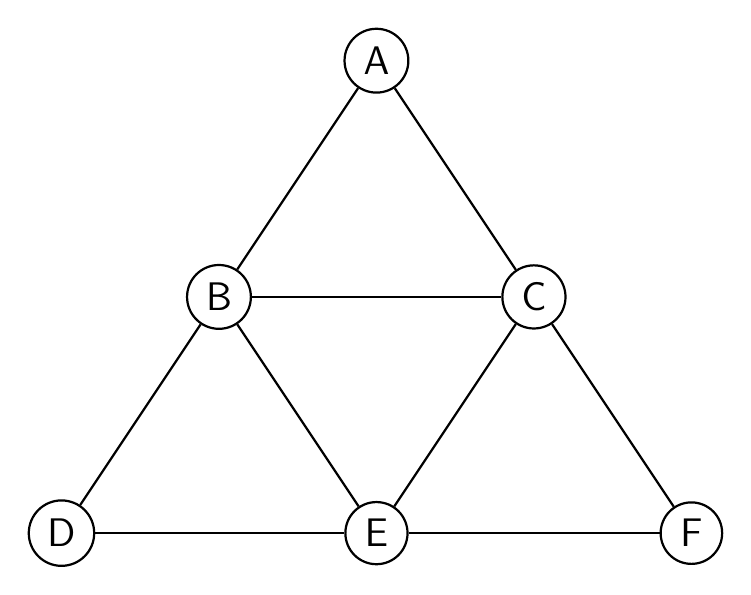
\begin{tikzpicture}[auto,node distance=3cm, every loop/.style={},thick,main node/.style={circle,draw,font=\sffamily\Large}]
        \node[main node] at (0, 2) (a) {A};
        \node[main node] at (-2, -1) (b) {B};
        \node[main node] at (2, -1) (c) {C};
        \node[main node] at (-4, -4) (d) {D};
        \node[main node] at (0, -4) (e) {E};
        \node[main node] at (4, -4) (f) {F};

        \path[every node/.style={font=\sffamily\small}]
            (a) edge[] node {} (b)
            (a) edge node {} (c)
            (b) edge node {} (c)
            (d) edge node {} (b)
            (d) edge node {} (e)
            (e) edge node {} (b)
            (e) edge node {} (c)
            (e) edge node {} (f)
            (f) edge node {} (c)
            ;
    \end{tikzpicture}
    \caption{Grafo $G$, foco do exemplo do algoritmo de Hierholzer}
\end{figure}

\sloppy O grafo apresentado possui uma grande quantidade de circuitos, por isso encontrar uma partição do mesmo em circuitos $C_1, C_2, \dots, C_k$ não é uma tarefa simples.
Uma possibilidade para este grafo é tomar $C_1 = \{A, B, C, A\}, C_2 = \{B, D, E, B\}, C_3 = \{C, E, F, C\}$, outra possibilidade é separar $G$ em dois circuitos apenas $C_1 = \{A, B, D, E, F, C, A\}, C_2 = \{B, E, C, B\}$.

\begin{figure}[H]
\centering
\begin{minipage}{.5\textwidth}
  \centering
    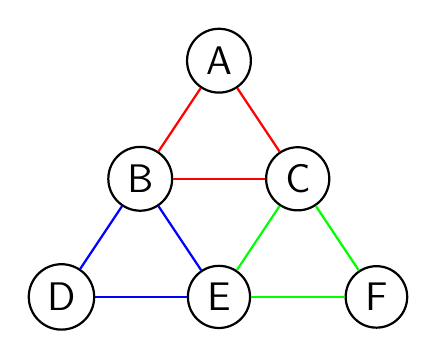
\begin{tikzpicture}[auto,node distance=3cm, every loop/.style={},thick,main node/.style={circle,draw,font=\sffamily\Large}]
        \node[main node] at (0, 1) (a) {A};
        \node[main node] at (-1, -.5) (b) {B};
        \node[main node] at (1, -.5) (c) {C};
        \node[main node] at (-2, -2) (d) {D};
        \node[main node] at (0, -2) (e) {E};
        \node[main node] at (2, -2) (f) {F};

        \path[every node/.style={font=\sffamily\small}]
            (a) edge[red] node {} (b)
            (a) edge[red] node {} (c)
            (b) edge[red] node {} (c)
            (d) edge[blue] node {} (b)
            (d) edge[blue] node {} (e)
            (e) edge[blue] node {} (b)
            (e) edge[green] node {} (c)
            (e) edge[green] node {} (f)
            (f) edge[green] node {} (c)
            ;
    \end{tikzpicture}
  \label{exCirc1}
\end{minipage}%
\begin{minipage}{.5\textwidth}
  \centering
    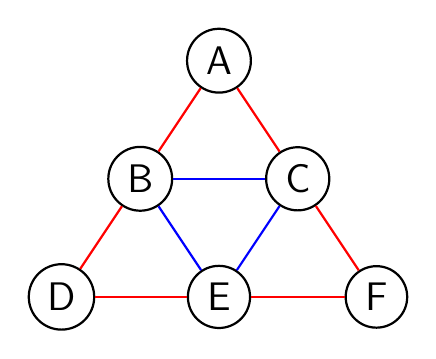
\begin{tikzpicture}[auto,node distance=3cm, every loop/.style={},thick,main node/.style={circle,draw,font=\sffamily\Large}]
        \node[main node] at (0, 1) (a) {A};
        \node[main node] at (-1, -.5) (b) {B};
        \node[main node] at (1, -.5) (c) {C};
        \node[main node] at (-2, -2) (d) {D};
        \node[main node] at (0, -2) (e) {E};
        \node[main node] at (2, -2) (f) {F};

        \path[every node/.style={font=\sffamily\small}]
            (a) edge[red] node {} (b)
            (a) edge[red] node {} (c)
            (b) edge[blue] node {} (c)
            (d) edge[red] node {} (b)
            (d) edge[red] node {} (e)
            (e) edge[blue] node {} (b)
            (e) edge[blue] node {} (c)
            (e) edge[red] node {} (f)
            (f) edge[red] node {} (c)
            ;
    \end{tikzpicture}
  \label{exCirc2}
\end{minipage}
    \caption{Dois exemplos de partição de $G$ em circuitos. Em vermelho representou-se $C_1$, em azul $C_2$ e em verde $C_3$.}
\end{figure}

Felizmente, não é necessário particionar o grafo nos circuitos para se determinar o circuito euleriano de $G$.

Simularemos nos próximos passos a busca em profundidade que o algoritmo realiza em $G$, tomando o vértice $A$ como o vértice inicial:

Neste exemplo, digamos que o trajeto inicial percorrido na busca é $\{A, B, C, A\}$.

\begin{figure}[H]
    \center
    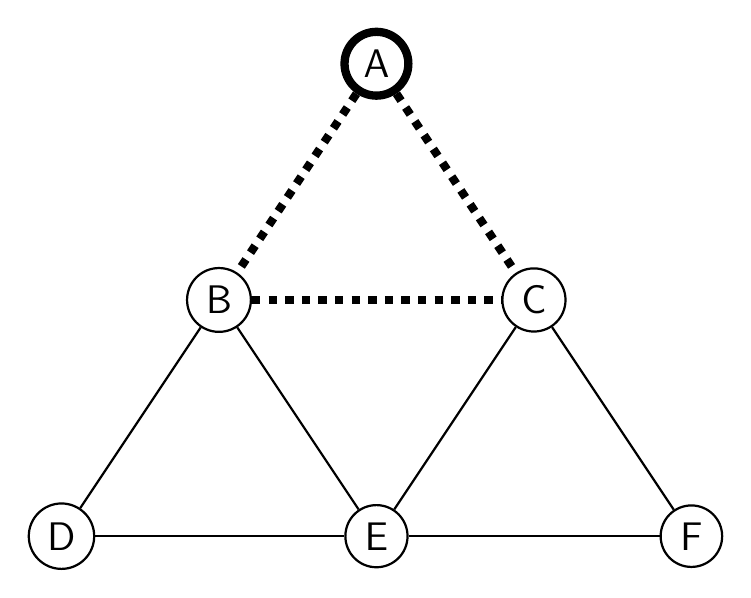
\begin{tikzpicture}[auto,node distance=3cm, every loop/.style={},thick,main node/.style={circle,draw,font=\sffamily\Large}]
        \node[main node, line width=3] at (0, 2) (a) {A};
        \node[main node] at (-2, -1) (b) {B};
        \node[main node] at (2, -1) (c) {C};
        \node[main node] at (-4, -4) (d) {D};
        \node[main node] at (0, -4) (e) {E};
        \node[main node] at (4, -4) (f) {F};

        \path[every node/.style={font=\sffamily\small}]
            (a) edge[line width=3, dashed] node {} (b)
            (a) edge[line width=3, dashed] node {} (c)
            (b) edge[line width=3, dashed] node {} (c)
            (d) edge node {} (b)
            (d) edge node {} (e)
            (e) edge node {} (b)
            (e) edge node {} (c)
            (e) edge node {} (f)
            (f) edge node {} (c)
            ;
    \end{tikzpicture}
    \caption{Representam-se pontilhadas as arestas percorridas na busca e em negrito o vértice atual da busca.}
\end{figure}

Após percorrido o caminho $\{A, B, C, A\}$ as arestas $AB, BC, BA$ são apagadas e a busca não consegue progredir para novas arestas a partir do vértice $A$.

Seja $T$ uma trilha inicialmente vazia.
Como $A$ não possui mais caminhos a se percorrer, adiciona-se o mesmo ao início da trilha $T$, e a busca continua recursivamente com o vértice $C$.

\begin{figure}[H]
    \center
    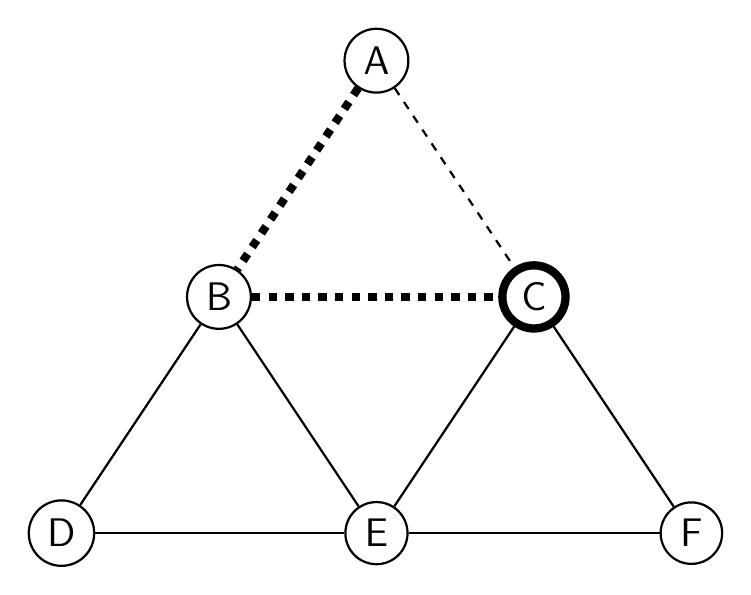
\begin{tikzpicture}[auto,node distance=3cm, every loop/.style={},thick,main node/.style={circle,draw,font=\sffamily\Large}]
        \node[main node] at (0, 2) (a) {A};
        \node[main node] at (-2, -1) (b) {B};
        \node[main node, line width=3] at (2, -1) (c) {C};
        \node[main node] at (-4, -4) (d) {D};
        \node[main node] at (0, -4) (e) {E};
        \node[main node] at (4, -4) (f) {F};

        \path[every node/.style={font=\sffamily\small}]
            (a) edge[line width=3, dashed] node {} (b)
            (a) edge[dashed] node {} (c)
            (b) edge[line width=3, dashed] node {} (c)
            (d) edge node {} (b)
            (d) edge node {} (e)
            (e) edge node {} (b)
            (e) edge node {} (c)
            (e) edge node {} (f)
            (f) edge node {} (c)
            ;
    \end{tikzpicture}
    \caption{Representam-se em negrito os arcos que ainda fazem parte da pilha de recursão da busca.}
\end{figure}

Seja $\{C, E, F, C\}$ o caminho percorrido na continuação da busca:


\begin{figure}[H]
    \center
    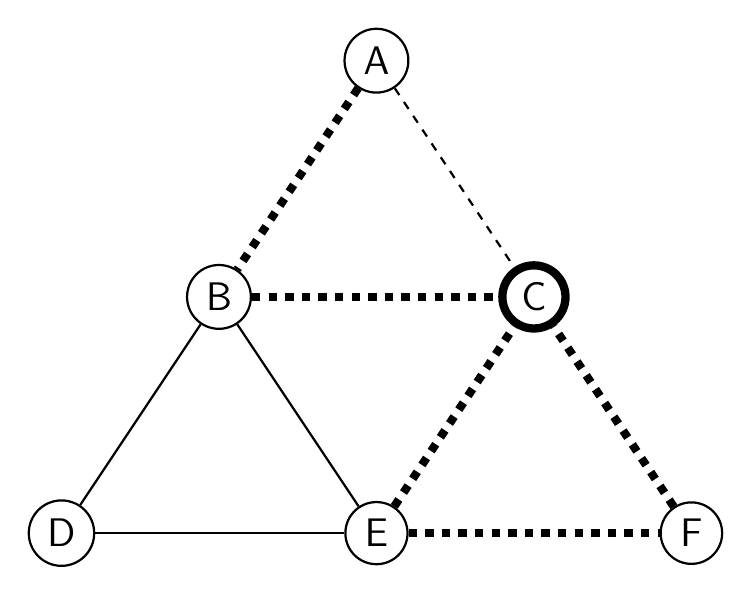
\begin{tikzpicture}[auto,node distance=3cm, every loop/.style={},thick,main node/.style={circle,draw,font=\sffamily\Large}]
        \node[main node] at (0, 2) (a) {A};
        \node[main node] at (-2, -1) (b) {B};
        \node[main node, line width=3] at (2, -1) (c) {C};
        \node[main node] at (-4, -4) (d) {D};
        \node[main node] at (0, -4) (e) {E};
        \node[main node] at (4, -4) (f) {F};

        \path[every node/.style={font=\sffamily\small}]
            (a) edge[line width=3, dashed] node {} (b)
            (a) edge[dashed] node {} (c)
            (b) edge[line width=3, dashed] node {} (c)
            (d) edge node {} (b)
            (d) edge node {} (e)
            (e) edge node {} (b)
            (e) edge[line width=3, dashed] node {} (c)
            (e) edge[line width=3, dashed] node {} (f)
            (f) edge[line width=3, dashed] node {} (c)
            ;
    \end{tikzpicture}
\end{figure}

De modo similar ao primeiro passo, adicionamos o vértice $C$ ao início de $T$ e voltamos, recursivamente ao vértice $F$. 

\begin{figure}[H]
    \center
    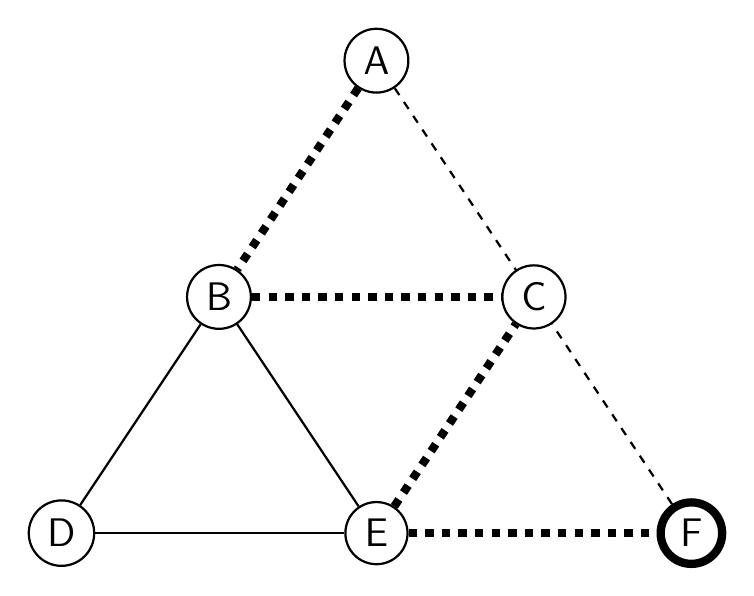
\begin{tikzpicture}[auto,node distance=3cm, every loop/.style={},thick,main node/.style={circle,draw,font=\sffamily\Large}]
        \node[main node] at (0, 2) (a) {A};
        \node[main node] at (-2, -1) (b) {B};
        \node[main node] at (2, -1) (c) {C};
        \node[main node] at (-4, -4) (d) {D};
        \node[main node] at (0, -4) (e) {E};
        \node[main node, line width=3] at (4, -4) (f) {F};

        \path[every node/.style={font=\sffamily\small}]
            (a) edge[line width=3, dashed] node {} (b)
            (a) edge[dashed] node {} (c)
            (b) edge[line width=3, dashed] node {} (c)
            (d) edge node {} (b)
            (d) edge node {} (e)
            (e) edge node {} (b)
            (e) edge[line width=3, dashed] node {} (c)
            (e) edge[line width=3, dashed] node {} (f)
            (f) edge[dashed] node {} (c)
            ;
    \end{tikzpicture}
\end{figure}

Como $F$ também não possui arestas, ele é adicionado ao início de $T$, e a busca volta ao vértice $E$.
Até o momento, $T = \{F, C, A\}$

\begin{figure}[H]
    \center
    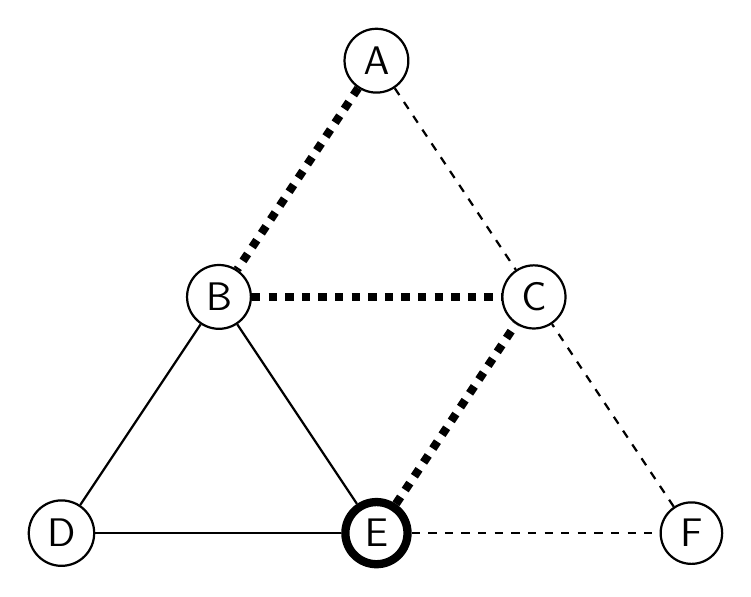
\begin{tikzpicture}[auto,node distance=3cm, every loop/.style={},thick,main node/.style={circle,draw,font=\sffamily\Large}]
        \node[main node] at (0, 2) (a) {A};
        \node[main node] at (-2, -1) (b) {B};
        \node[main node] at (2, -1) (c) {C};
        \node[main node] at (-4, -4) (d) {D};
        \node[main node, line width=3] at (0, -4) (e) {E};
        \node[main node] at (4, -4) (f) {F};

        \path[every node/.style={font=\sffamily\small}]
            (a) edge[line width=3, dashed] node {} (b)
            (a) edge[dashed] node {} (c)
            (b) edge[line width=3, dashed] node {} (c)
            (d) edge node {} (b)
            (d) edge node {} (e)
            (e) edge node {} (b)
            (e) edge[line width=3, dashed] node {} (c)
            (e) edge[dashed] node {} (f)
            (f) edge[dashed] node {} (c)
            ;
    \end{tikzpicture}
\end{figure}

A partir de $E$ a busca continua no caminho, por exemplo, $\{E, D, B, E\}$.

\begin{figure}[H]
    \center
    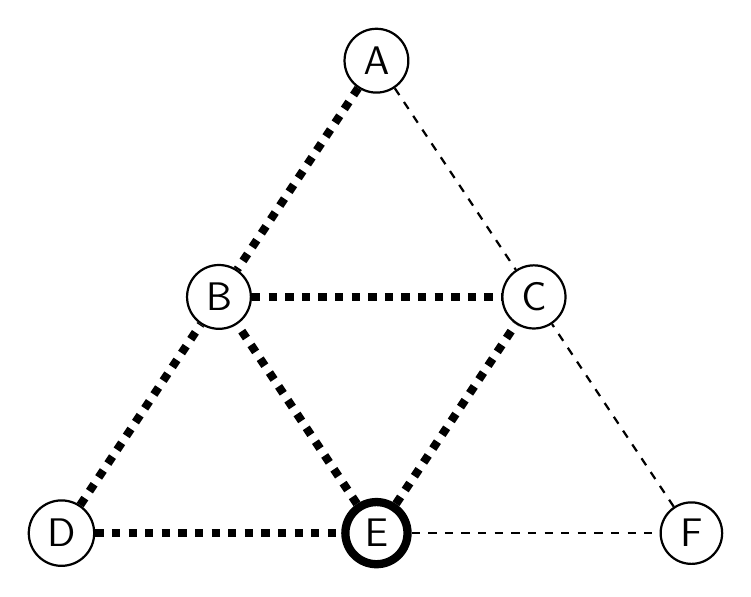
\begin{tikzpicture}[auto,node distance=3cm, every loop/.style={},thick,main node/.style={circle,draw,font=\sffamily\Large}]
        \node[main node] at (0, 2) (a) {A};
        \node[main node] at (-2, -1) (b) {B};
        \node[main node] at (2, -1) (c) {C};
        \node[main node] at (-4, -4) (d) {D};
        \node[main node, line width=3] at (0, -4) (e) {E};
        \node[main node] at (4, -4) (f) {F};

        \path[every node/.style={font=\sffamily\small}]
            (a) edge[line width=3, dashed] node {} (b)
            (a) edge[dashed] node {} (c)
            (b) edge[line width=3, dashed] node {} (c)
            (d) edge[line width=3, dashed] node {} (b)
            (d) edge[line width=3, dashed] node {} (e)
            (e) edge[line width=3, dashed] node {} (b)
            (e) edge[line width=3, dashed] node {} (c)
            (e) edge[dashed] node {} (f)
            (f) edge[dashed] node {} (c)
            ;
    \end{tikzpicture}
\end{figure}

Como todas as arestas de $G$ foram percorridas, a busca realiza, nos próximos passos, uma série de retornos, sempre adicionando à $T$ o vértice atual da busca.

\begin{figure}[H]
\centering
\begin{minipage}{.5\textwidth}
  \centering
    \scalebox{.7}{
        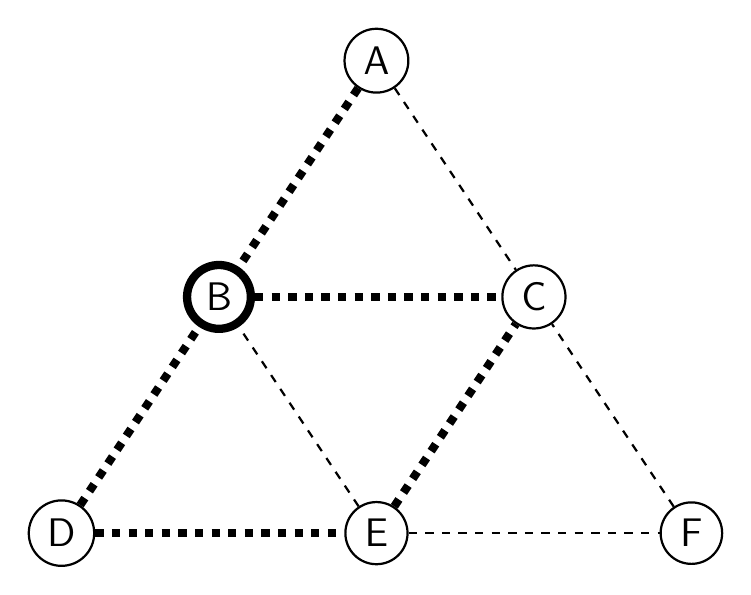
\begin{tikzpicture}[auto,node distance=3cm, every loop/.style={},thick,main node/.style={circle,draw,font=\sffamily\Large}]
        \node[main node] at (0, 2) (a) {A};
        \node[main node, line width=3] at (-2, -1) (b) {B};
        \node[main node] at (2, -1) (c) {C};
        \node[main node] at (-4, -4) (d) {D};
        \node[main node] at (0, -4) (e) {E};
        \node[main node] at (4, -4) (f) {F};

        \path[every node/.style={font=\sffamily\small}]
            (a) edge[line width=3, dashed] node {} (b)
            (a) edge[dashed] node {} (c)
            (b) edge[line width=3, dashed] node {} (c)
            (d) edge[line width=3, dashed] node {} (b)
            (d) edge[line width=3, dashed] node {} (e)
            (e) edge[dashed] node {} (b)
            (e) edge[line width=3, dashed] node {} (c)
            (e) edge[dashed] node {} (f)
            (f) edge[dashed] node {} (c)
            ;
        \end{tikzpicture}
    }
\end{minipage}%
\begin{minipage}{.5\textwidth}
  \centering
    \scalebox{.7}{
        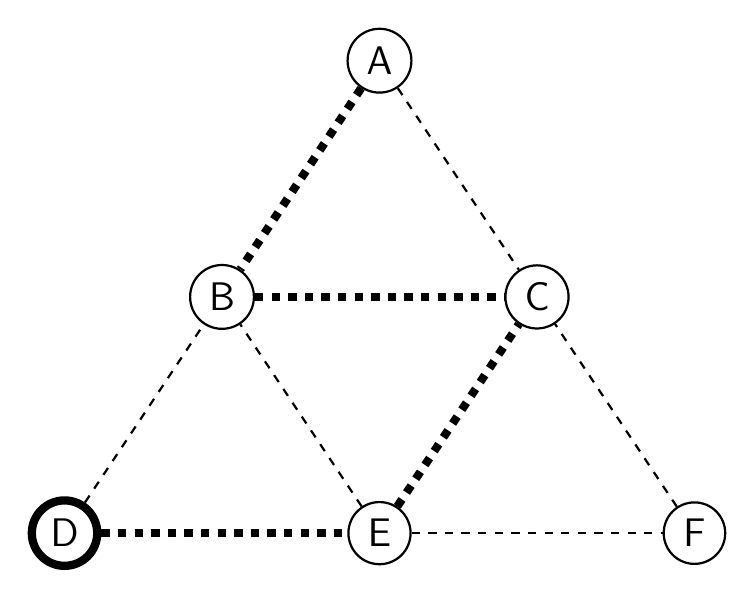
\begin{tikzpicture}[auto,node distance=3cm, every loop/.style={},thick,main node/.style={circle,draw,font=\sffamily\Large}]
        \node[main node] at (0, 2) (a) {A};
        \node[main node] at (-2, -1) (b) {B};
        \node[main node] at (2, -1) (c) {C};
        \node[main node, line width=3] at (-4, -4) (d) {D};
        \node[main node] at (0, -4) (e) {E};
        \node[main node] at (4, -4) (f) {F};

        \path[every node/.style={font=\sffamily\small}]
            (a) edge[line width=3, dashed] node {} (b)
            (a) edge[dashed] node {} (c)
            (b) edge[line width=3, dashed] node {} (c)
            (d) edge[dashed] node {} (b)
            (d) edge[line width=3, dashed] node {} (e)
            (e) edge[dashed] node {} (b)
            (e) edge[line width=3, dashed] node {} (c)
            (e) edge[dashed] node {} (f)
            (f) edge[dashed] node {} (c)
            ;
        \end{tikzpicture}
    }
\end{minipage}%
\end{figure}

\begin{figure}[H]
\centering
\begin{minipage}{.5\textwidth}
  \centering
    \scalebox{.7}{
        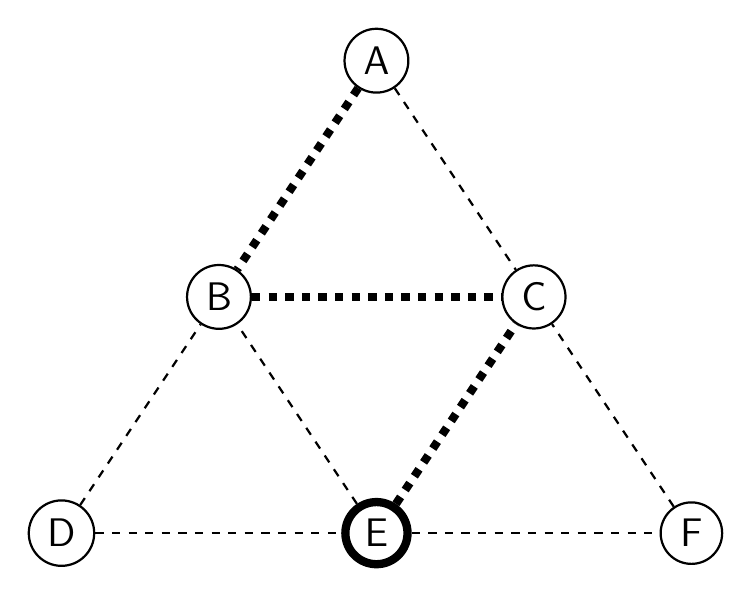
\begin{tikzpicture}[auto,node distance=3cm, every loop/.style={},thick,main node/.style={circle,draw,font=\sffamily\Large}]
        \node[main node] at (0, 2) (a) {A};
        \node[main node] at (-2, -1) (b) {B};
        \node[main node] at (2, -1) (c) {C};
        \node[main node] at (-4, -4) (d) {D};
        \node[main node, line width=3] at (0, -4) (e) {E};
        \node[main node] at (4, -4) (f) {F};

        \path[every node/.style={font=\sffamily\small}]
            (a) edge[line width=3, dashed] node {} (b)
            (a) edge[dashed] node {} (c)
            (b) edge[line width=3, dashed] node {} (c)
            (d) edge[dashed] node {} (b)
            (d) edge[dashed] node {} (e)
            (e) edge[dashed] node {} (b)
            (e) edge[line width=3, dashed] node {} (c)
            (e) edge[dashed] node {} (f)
            (f) edge[dashed] node {} (c)
            ;
        \end{tikzpicture}
    }
\end{minipage}%
\begin{minipage}{.5\textwidth}
  \centering
    \scalebox{.7}{
        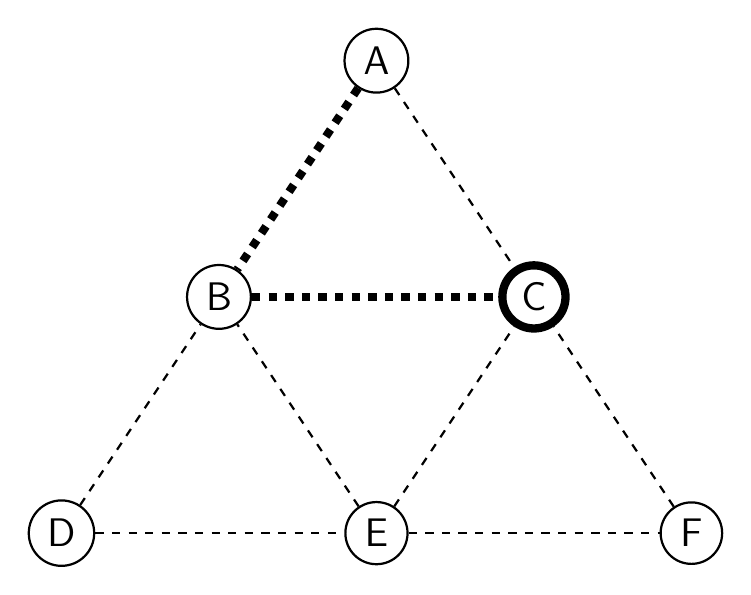
\begin{tikzpicture}[auto,node distance=3cm, every loop/.style={},thick,main node/.style={circle,draw,font=\sffamily\Large}]
        \node[main node] at (0, 2) (a) {A};
        \node[main node] at (-2, -1) (b) {B};
        \node[main node, line width=3] at (2, -1) (c) {C};
        \node[main node] at (-4, -4) (d) {D};
        \node[main node] at (0, -4) (e) {E};
        \node[main node] at (4, -4) (f) {F};

        \path[every node/.style={font=\sffamily\small}]
            (a) edge[line width=3, dashed] node {} (b)
            (a) edge[dashed] node {} (c)
            (b) edge[line width=3, dashed] node {} (c)
            (d) edge[dashed] node {} (b)
            (d) edge[dashed] node {} (e)
            (e) edge[dashed] node {} (b)
            (e) edge[dashed] node {} (c)
            (e) edge[dashed] node {} (f)
            (f) edge[dashed] node {} (c)
            ;
        \end{tikzpicture}
    }
\end{minipage}%
\end{figure}

\begin{figure}[H]
\centering
\begin{minipage}{.5\textwidth}
  \centering
    \scalebox{.7}{
        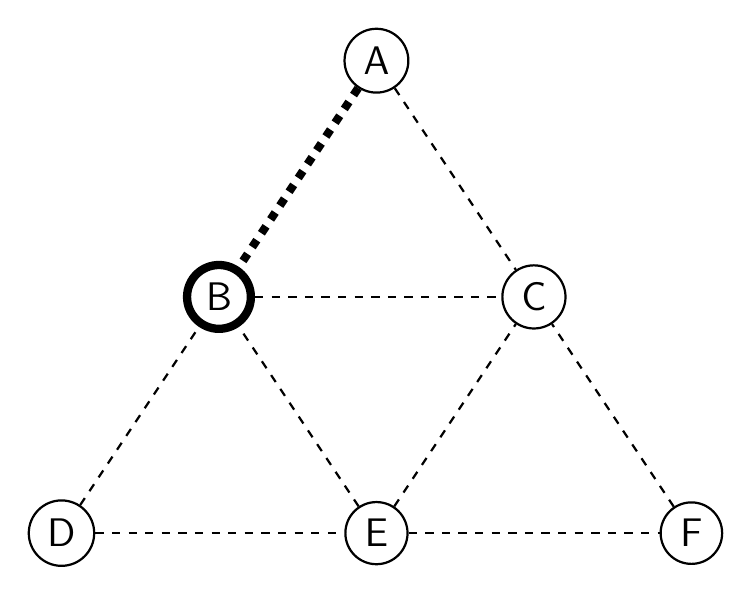
\begin{tikzpicture}[auto,node distance=3cm, every loop/.style={},thick,main node/.style={circle,draw,font=\sffamily\Large}]
        \node[main node] at (0, 2) (a) {A};
        \node[main node, line width=3] at (-2, -1) (b) {B};
        \node[main node] at (2, -1) (c) {C};
        \node[main node] at (-4, -4) (d) {D};
        \node[main node] at (0, -4) (e) {E};
        \node[main node] at (4, -4) (f) {F};

        \path[every node/.style={font=\sffamily\small}]
            (a) edge[line width=3, dashed] node {} (b)
            (a) edge[dashed] node {} (c)
            (b) edge[dashed] node {} (c)
            (d) edge[dashed] node {} (b)
            (d) edge[dashed] node {} (e)
            (e) edge[dashed] node {} (b)
            (e) edge[dashed] node {} (c)
            (e) edge[dashed] node {} (f)
            (f) edge[dashed] node {} (c)
            ;
        \end{tikzpicture}
    }
\end{minipage}%
\begin{minipage}{.5\textwidth}
  \centering
    \scalebox{.7}{
        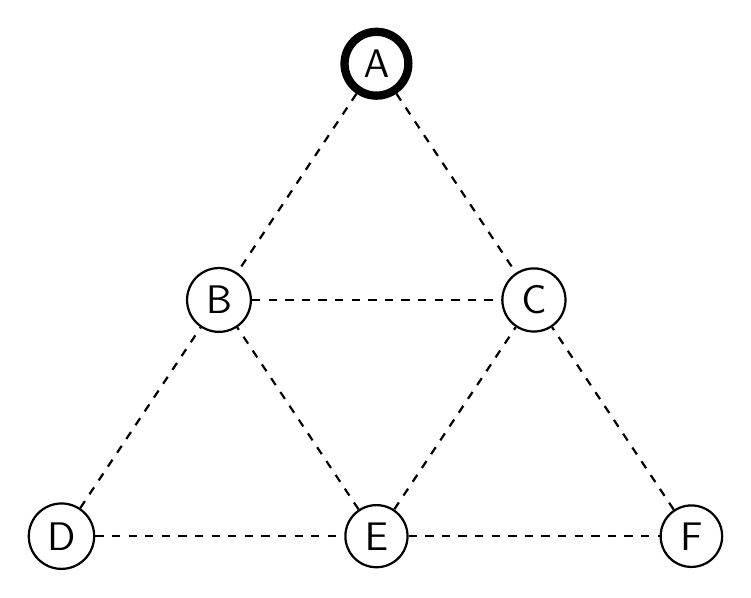
\begin{tikzpicture}[auto,node distance=3cm, every loop/.style={},thick,main node/.style={circle,draw,font=\sffamily\Large}]
        \node[main node, line width=3] at (0, 2) (a) {A};
        \node[main node] at (-2, -1) (b) {B};
        \node[main node] at (2, -1) (c) {C};
        \node[main node] at (-4, -4) (d) {D};
        \node[main node] at (0, -4) (e) {E};
        \node[main node] at (4, -4) (f) {F};

        \path[every node/.style={font=\sffamily\small}]
            (a) edge[dashed] node {} (b)
            (a) edge[dashed] node {} (c)
            (b) edge[dashed] node {} (c)
            (d) edge[dashed] node {} (b)
            (d) edge[dashed] node {} (e)
            (e) edge[dashed] node {} (b)
            (e) edge[dashed] node {} (c)
            (e) edge[dashed] node {} (f)
            (f) edge[dashed] node {} (c)
            ;
        \end{tikzpicture}
    }
\end{minipage}%
\end{figure}

\sloppy Nesta série de retornos são adicionados ao início de $T$ os vértices $E, B, D, E, C, B, A$, um a um.

Finalizando-se a simulação do algoritmo temos a seguinte trilha $T$:

\[
    T = \{A, B, C, E, D, B, E, F, C, A\}
\]

Como pode-se conferir, a trilha $T$ construída é um circuito euleriano de $G$.


Segue agora a implementação do algoritmo de Hierholzer em C++ para digrafos:

\lstinputlisting[language=c++,firstline=13,lastline=21]{../code/euler-digrafo.cpp}

Optou-se nesta implementação pelo uso de uma pilha para o armazenamento da lista de adjacências $adj$, pois assim é possível apagar facilmente os arcos já percorridas na busca.


Para que tal função retorne corretamente uma trilha euleriana em grafos que não possuem circuito euleriano, é necessário que a primeira chamada de $trilha\_euleriana$ tenha como parâmetro $u$ o vértice cujo grau de saída é maior que seu grau de entrada, ou seja o vértice que será necessariamente o ínico da trilha euleriana.

Como em cada iteração deste algoritmo um arco é deletado, o número máximo de iterações que ele pode realizar é limitado pelo número de arcos de um digrafo, sendo assim o mesmo possui complexidade $\mathcal{O}(|E|)$.

Pode-se adaptar este algoritmo para grafos não direcionados mudando o modo como arestas são apagadas.
O algoritmo mostrado não funciona para grafos não direcionados pois o mesmo trata cada sentido de uma aresta $uv$ como dois arcos separados, $u \rightarrow v$ e $v \rightarrow u$. 
Sendo assim, quando uma aresta é deletada, digamos $u \rightarrow v$, seu arco reverso $v \rightarrow u$, não é deletado automaticamente.

Para corrigir isto, pode-se criar um identificador único para cada aresta (igual para os dois sentidos de uma mesma aresta) que pode ser utilizado para marcar as arestas já percorridas na busca em profundidade \footnote{Segue uma implementação do algoritmo para grafos não direcionados, que utiliza as modificações descritas \href{https://github.com/gafeol/chinese-postman/blob/master/code/euler-grafo.cpp}{https://github.com\-/gafeol\-/chinese-postman\-/blob/master\-/code/euler-grafo.cpp}}. 

